\chapter{Кимврская война, 113-101г до н.э}



\textbf{Поговорим про самое страшное для римлян вторжение со времен Ганнибала.} Никто ещё не заходил в противостоянии с Республикой так далеко, и, что ещё интереснее, никто не смог заставить римлян менять свой упорядоченный быт так основательно. Менять чтобы выжить. Пожалуй, римляне очень сильно отвыкли от того, что им надо что-то делать для собственного выживания, вопрос всегда стоял в каких-то профитах или потерях. И они менялись, причем кардинально. Итак, встречайте наших сегодняшних гостей, причину маринских реформ и просто хороших ребят, германские племенные союзы кимвров и тевтонов. Которые сидели себе гдет на севере, сидели, а потом взяли и откочевали на юг, прямо на порог к потихоньку разлагающейся от безделья Римской республике.


Угроза германцев была очень серьезной, они снялись с насиженных мест и огромной массой (источники говорят о полумилионе, но это явно преувеличение) двинулись на юг. Первая встреча кимвров с римлянами случилась в восточных предгорьях Альп, недалеко от Нореи в 113г до н.э. Римляне внезапно напали на достаточно миролюбиво настроенных варваров, но потерпели поражение и были рассеяны.

\begin{figure}[h!tb]
	\centering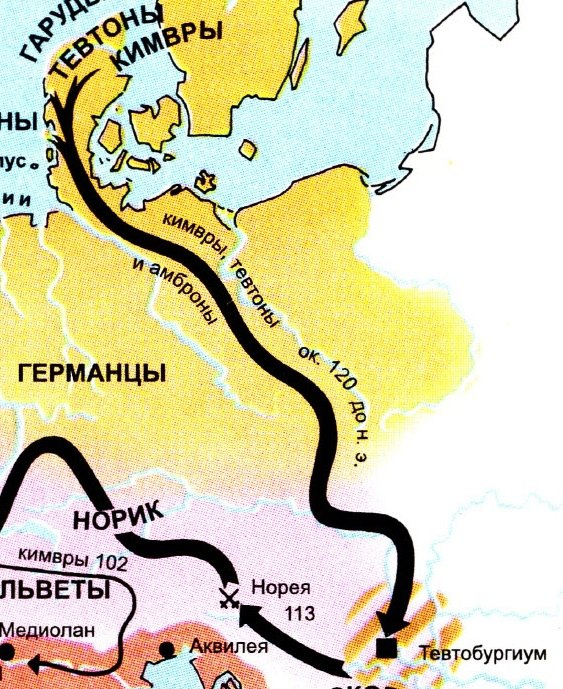
\includegraphics[scale=0.45]{kimres/1574757799180321900.png}
	\label{fig:kimr1} % Unique label used for referencing the figure in-text
	%\addcontentsline{toc}{figure}{Figure \ref{fig:placeholder}} % Uncomment to add the figure to the table of contents
	\caption{Первая встреча двух сборных. }
\end{figure}




После чего орда, через земли гельветов (современная Швейцария), попутно обрастая примыкающими к ним горными народностями, вытекла на равнины Трансальпийской Галлии и начала там настоящую бойню против достаточно воинственных, но неорганизованных и очень давно толком не воевавших галлов. Римляне из римской провинции Провинция (современный Прованс, также иногда называется Нарбонской Галлией) в ужасе следили за идущей в центральной Галлии мясорубкой и наращивали военное присутствие. В 109 и 107 годах ещё две крупные римские армии были разгромлены на границе, и хоть варвары не пытались вторгаться в, собственно, Провинцию, ситуация становилась всё более критической. Кимвры собирали разрозненные галльские народности, выжирая под собой землю как саранча. Становилось очевидно, что следующей целью вторжения будут уже непосредственно римские владения, и если орду не остановить, она перейдет через Альпы и просто сметет всё на своем пути.


Попутно в Африке шла Югуртинская война (112-105г до н.э.), на которой находились и приходили к успеху Гай Марий и Луций Корнелий Сулла. И хоть это не имеет прямого отношения к Кимврской войне, но немалую часть римской армии пришлось перебросить туда, а набираемые взамен, де-факто, ополчения были недостаточно качественны. Да и резерв кадровых офицеров тоже был вычерпан. Во многом поэтому такие вчерашние школьники как Серторий делали почти мгновенную карьеру до младших командиров.


В 106г до н.э. Сенат собирает две армии, полностью мобилизуя свои резервы в Италии. И в этот момент вмешалась чисто классовая неприязнь внутри римского истеблишмента: ни одна из партий не хотела видеть конкурента во главе столь внушительной силы. Поэтому оптиматы продвинули на должность проконсула Провинции, Квинта Цепиона. Ему была отдана одна из армий. Популяры в ответ продвинули в консулы на 105г до н.э. Гнея Маллия Максима, человека не слишком знатного происхождения, но, видимо, больших талантов, раз уж сумел пролезть так высоко. Ему досталась вторая армия и формальное командование всей операцией.


А в Галлии в этот момент собиралась орда. Сожравшие всё что только можно было сожрать (лишь белги (современные Бельгия с Голландией) кое-как отбились, в основном потому, что сами мало чем от германцев отличались) германцы мобилизовали ресурсы захваченных народов и собрались двигаться на юг, к новым целям. И идти им было особенно некуда, так как и Испанию и Италию защищали естественные горные преграды (Пиренеи и Альпы соответственно) для столь крупных сил непроходимые. Но вот вдоль побережья Средиземного моря можно было без проблем вторгнуться в оба этих региона. А на пути к морю стояла всё та же римская Провинция, поэтому решающее сражение становилось просто безальтернативным.


\begin{figure}[h!tb]
	\centering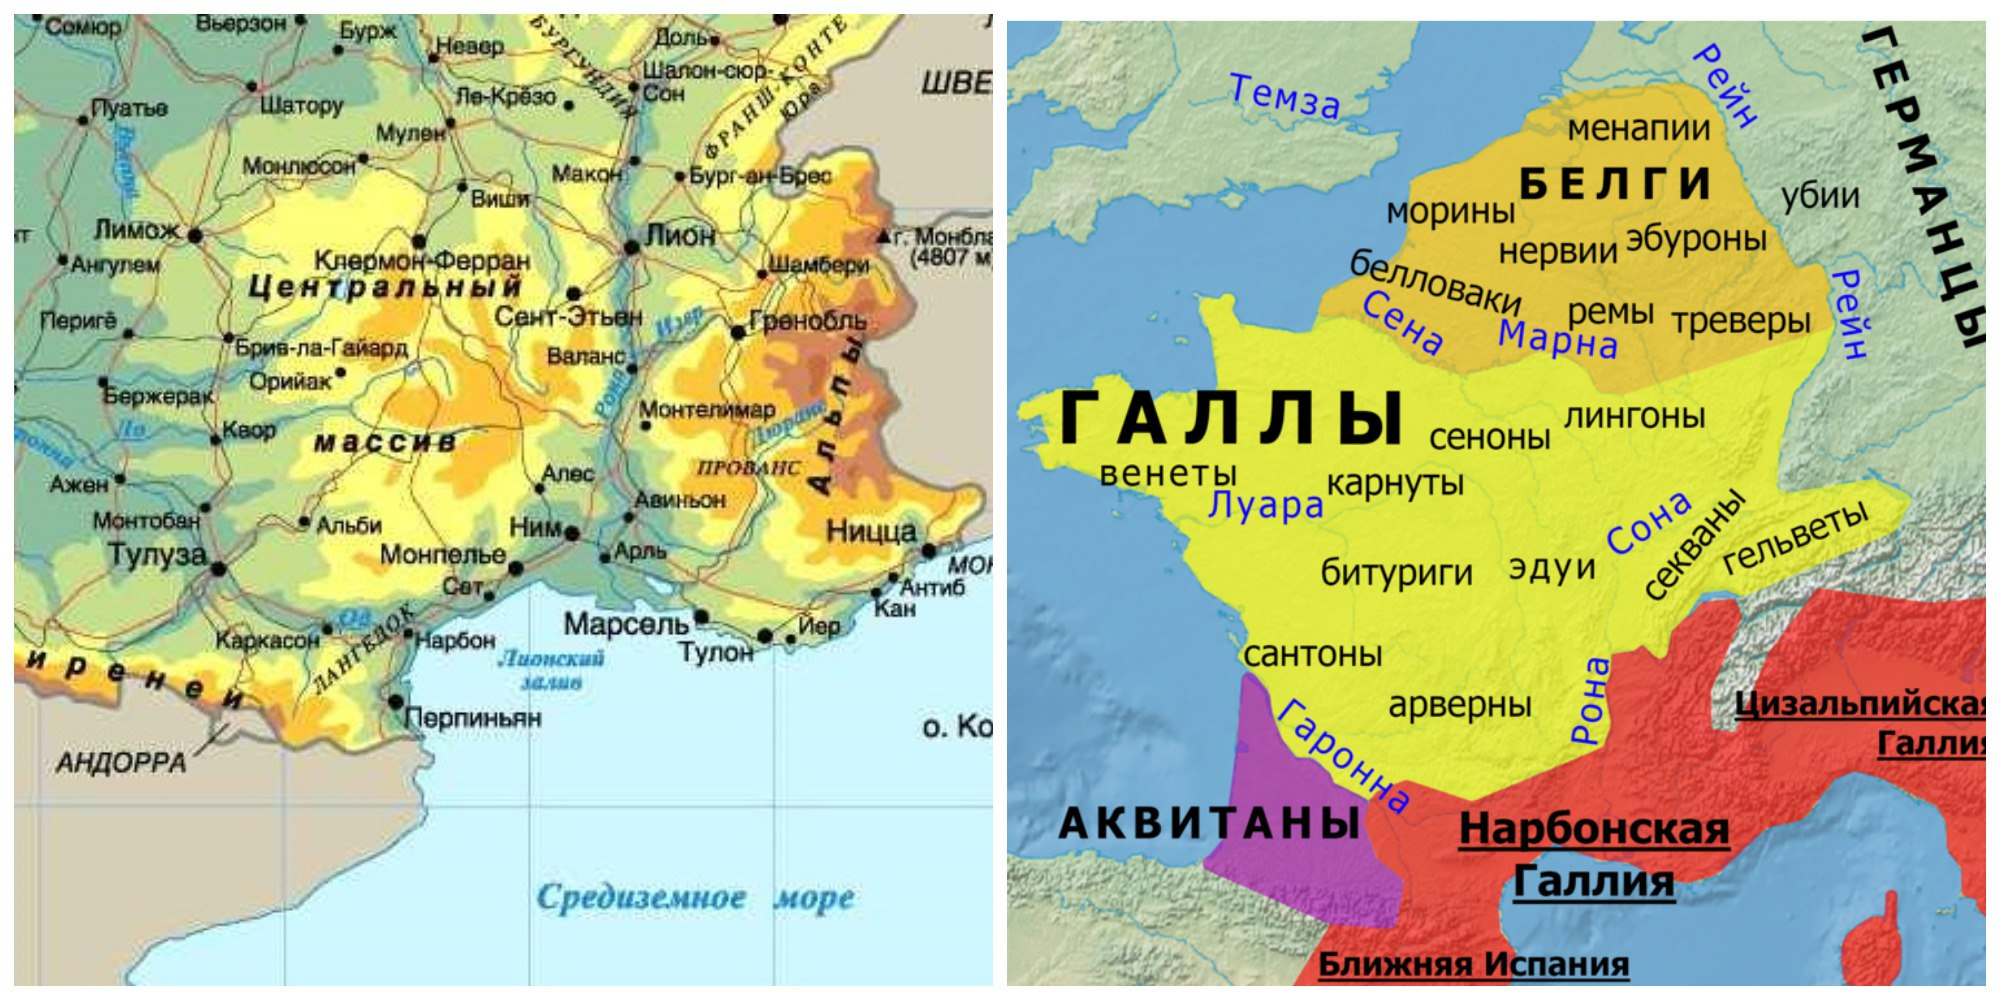
\includegraphics[scale=0.25]{kimres/1574757993132297819.png}
	\label{fig:kimr2} % Unique label used for referencing the figure in-text
	%\addcontentsline{toc}{figure}{Figure \ref{fig:placeholder}} % Uncomment to add the figure to the table of contents
	\caption{На первой карте современная физическая география юга Франции.Тут можно наблюдать такую своеобразную воронку между Альпами и Центральным Массивом. И два направления вдоль Средиземного Моря, одно в Италию, второе в Испанию. И там и там между горами и морем есть несколько километров равнины, пригодной для прохода десятков тысяч человек единовременно. Лезть с такой толпой в горы для варваров было самоубийством, поэтому римляне и очковали. Прекрасно понимали, что на юг всего один маршрут, и он идет через них, через Нарбонскую Галлию (то есть Провинцию)}
\end{figure}


Прибывшим в начале года в Провинцию римским военачальникам пришлось подавить несколько мятежей местных племен, почуявших что власть Рима шатается, после чего они стали готовиться к отражению набега. Ближе к осени германцы начали свою миграцию. И тут, собственно, как гнойник вскрылся конфликт между двумя военачальниками. Являющийся консулом Максим был формально старше, но при этом находился на территории провинции, в которой Цепион был проконсулом. Кроме того, Цепион был куда более знатной персоной, а Максим — "новым человеком", которому зашкварно подчиняться. В итоге к началу вторжения отношения между двумя военачальниками настолько накалились, что ни о каком сотрудничестве говорить не приходилось, они даже лагеря поставили в серьезном отдалении друг от друга. Но, тем не менее, римляне собрали значительные силы, историки говорят про 80к легионеров и 40к войск поддержки, расположившихся на северном берегу реки Родан (тоесть переправились через реку и оставили её в тылу). Поэтому когда германцы подошли к реке, где их поджидали римляне, то предпочли вступить в переговоры с Максимом (как старшим по званию).


Сами германцы утверждали, что им надо в Испанию, римлян они трогать не хотят и вообще не понимают в чем проблема. И неизвестно к чему бы эти переговоры привели (хотя скорее всего ни к чему, так как для Максима пустить орду в римскую Испанию было бы политическим самоубийством), но в этот момент у Цепиона что-то щелкнуло в голове (могу предположить, что случилось непроизвольное возгорание от того что Максим начал с германцами переговоры а его не позвал) и он приказал своим войскам внезапно атаковать германцев всеми силами. Максим к этому готов не был, да и германцы охренели, но среагировали быстрее, и пока консул тупил, пытаясь понять что происходит — окружили, прижали к реке и полностью разгромили войска Цепиона. Чуть позже то же самое провернули и с армией Максима.


Потери исчислялись десятками тысяч человек, погибло очень много знати всех сортов и расцветок, и последняя римская армия в Италии. Хотя Максим и Цепион спаслись, и смогли отойти в Рим, но предстали перед судом и были приговорены к изгнанию, закончив свою политическую карьеру навсегда. Германцы же не обманули, и после разграбления Провинции разделились на три тактические группы. Две двинулись в Испанию, разными маршрутами, а третья вернулась обратно в Галлию, где продолжила разграбление региона. В Риме выдохнули, немедленный неотвратимый пиздец откладывался на некоторое время.


Тогда же, в год разгрома римлян германцами, Гай Марий закончил войну в Африке с царем Югуртой. Самого царя отвезли в Рим и вскоре казнили. Но главное, высвободилась прекрасно обученная и опытная армия Мария, вместе со своим полководцем. На фоне событий на северных рубежах, африканские новости были лучиком света в полном хтонического ужаса 105г до н.э, поэтому Сенат особо не возражал, когда "новый человек" Марий занял консульскую должность (которую будет занимать ещё пять раз подряд, что было против законов, но всем пофигу) и превратился в нечто вроде военного диктатора всей Италии. Начались так называемые "Марианские Реформы" по превращению армии из полисного ополчения в античный аналог ЧВК. Он начал с этим экспериментировать ещё в Африке, а тут ему предстояло всю Республику переформатировать под свои стандарты. Более подробно про эти реформы можно почитать тут.


Но краткая суть такова: снятие имущественного ценза и гражданского ценза для рекрутов, гражданство, участок земли и выходное пособие для тех кто доживет до демобилизации, централизованное снабжение армии вооружением и припасами за счет казны, выплата жалования солдатам, право солдат на долю в трофеях после боя, и, пожалуй, всё. Причем всё это надо было делать в пожарном порядке, пока германские слоупоки не вернулись из своего турне по испанским курортам и не полезли через Альпы. Марий получил карт-бланш от Сената на все нужные действия, плюс притащил из Африки несколько тысяч своих ветеранов, способных стать костяком новой армии. Но этого было всё равно недостаточно, поэтому вводились некоторые чрезвычайные меры, вроде вербовки в армию гладиаторов (то есть, де-факто рабов) в качестве инструкторов, а молодым людям до 25 лет было запрещено покидать Италию под любыми предлогами, и их массово гребли в армию. Плюс, Марий активно сгребал в армию союзные Риму италийские народности, обещая целым общинам гражданские права если они выполнят его норму по рекрутам. Те радостно соглашались и быстро собирали нужное количество. В тот момент гражданство для целой общины освобождало от основного налога и позволяло принимать участие в римской политической жизни. Предложение было щедрым, но и положение критическим. Запомните этот момент, это важно.


В общем, таким макаром, весь в делах и заботах, Марий отмобилизовал нужное себе количество рекрутов, обмундировал их за счет казны и выдрессировал по собственноручно разработанной методике, суть которой выражается древней максимой "чем бы солдат не занимался, лишь бы заебался". Бесконечно гоняя солдатенов по стране, заставляя строить и снимать лагеря, проводя бесконечные учения, ну и так далее. Через пару месяцев такой жизни марианская армия уже боялась своего командира сильнее чем германцев и молилась чтобы началась война, что и требовалось. И война началась.


Орда кимвров, после разгрома римских армий свернувшая в Испанию, вернулась, в общем и целом, отмудоханная и ничего там не добившаяся. Варвары опять проявили топографический кретинизм, и вместо того чтобы идти вдоль побережья, выжигая никем толком не защищаемые богатейшие римские колонии, за каким-то хреном поперлись вглубь полуострова, где проживали племена кельтиберов. О них мы потом обязательно подробно поговорим, но пока что поверьте мне на слово — жили там люди ещё более ебанутые чем сами германцы, при этом находились у себя дома, в горах, поэтому кимвры там плотнейшим образом завязли. А когда поняли что никаких быстрых успехов не будет и они просто тут все погибнут, то повернули назад, к более богатым и более травоядным галлам и римлянам. Так чудесное провидение спасло римскую Испанию от тотального уничтожения. Однако с самой Италией такой фокус прокатить не мог, тут уж либо римляне смогут защитить свой полуостров, либо их просто сотрут в порошок. Плюс, из Германии пришло второе крупное племя, тевтоны, а значит силы противника не просто не уменьшились, а даже наоборот. Да и сами галлы, кто вовремя сдался кимврам и поэтому пережил резню, тоже собирались поучаствовать в походе. В общем, собиралось нечто очень огромное, права на ошибку у Мария не было.


К счастью, варвары либо пересрались между собой (что типично для варваров), либо просто не считали, после последней встречи, римлян за противников, но они решили разделить свои силы на три группы. Первую должны были возглавить недавно прибывшие тевтоны, которые двигались в Италию с запада, вдоль побережья, по самой короткой дороге. Кимвры же должны были пересечь Альпы со стороны Дуная, с востока. Третья группа непонятно что хотела делать, так что будем считать что это стратегический резерв и вторая волна вторжения.


Марий тоже разделил свои силы на две части, и опять из-за римской политоты. За три года после прошлого поражения, фракция оптиматов немного отошла от шока и в 102г до н.э. смогла продвинуть в консулы своего человека, Квинта Лутация Катула, который был женат на сестре Цепиона. В итоге, когда варвары начали вторжение с двух направлений, Марий со своей армией выдвинулся навстречу двигающимся прямо на Рим тевтонам, а Катул должен был попытаться разбить или хотя-бы задержать идущих обходным путем кимвров. С армией Катула был и Луций Корнелий Сулла, ещё один герой Африканской войны, хоть и находящийся, пока что, в тени славы Мария. Тут может быть два варианта. Как мы знаем, где-то в это время отношения Мария с Суллой очень сильно охладели, но непонятно, до или после 102 года. Сулла вполне мог сам уйти поддерживать своего коллегу Катула из политических соображений (чтобы он, значит, не просрал все битвы и не было так же стыдно, как за Цепиона), или его мог направить сам Марий, для того чтобы Сулла не дал Катулу просрать всю армию пока Марий разбирается с тевтонами. Но в любом случае, так как у Катула военного опыта нихрена не было, его командование было очень формальным, рулил боевыми действиями на этом направлении Сулла и его офицеры, что и требовалось Марию.


Битва с тевтонами произошла при Аквах Секстиевых, городе недалеко от Мессалии в Нарбонской Галлии. Марий постарался сначала преодолеть ужас своих солдат перед варварами, просто встав лагерем на их пути. Орда пыталась сманеврировать и пройти мимо, но Марий вынудил тех начать штурм и три дня отбивал атаки не умеющих в осадное дело тевтонов. После этого вождь превратил долбится в стены и повел свою армию дальше, а Марий держался от него в некотором отдалении и периодически наносил удары по арьергарду. Спешить ему было особо некуда, орда двигалась медленно и была неповоротливой.


Когда Марий посчитал что его воины уже достаточно потренировались, то занял выгодную позицию на холме, и послал свою кавалерию кошмарить германцев. Те среагировали так, как он и предполагал, выдвинулись из своей стоянки неорганизованными толпами, и несколько километров бежали до позиций Мария, а затем ещё лезли на холм под обстрелом пилумами и стрелами. Ну и началась битва, где в несколько раз уступающие в численности римляне за счет превосходства в вооружении и организованности, плюс за счет позиции, смогли вымотать германцев и атаки тех ослабели. В этот момент Марий приказал начать общую контратаку, и его относительно свежие легионеры сбросили германцев по склону холма, а стоящие до этого времени в засаде пол легиона нанесли тем удар в тыл. После чего началось повальное бегство и резня, флауэрс виктори.


\begin{figure}[h!tb]
	\centering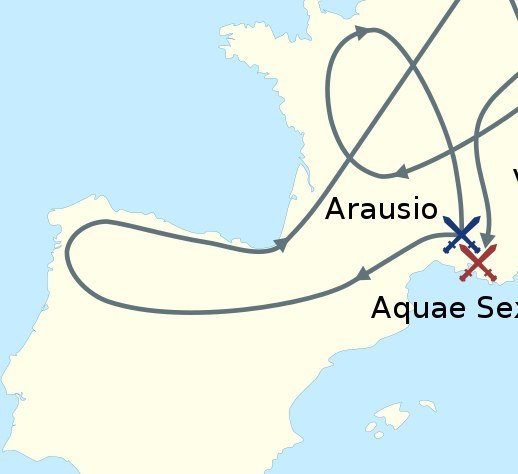
\includegraphics[scale=0.6]{kimres/1574758535182364019.png}
	\label{fig:kimr3} % Unique label used for referencing the figure in-text
	%\addcontentsline{toc}{figure}{Figure \ref{fig:placeholder}} % Uncomment to add the figure to the table of contents
	\caption{Как можно заметить, битва при Араузионе (где римляне потерпели свое крупнейшее поражение. На карте синим цветом) и битва при Аквах Секстиевых (Где Марий попячил германцев. На карте красным) происходили практически по соседству. Я уже выше говорил о том, что Нарбонская Галлия это трехсторонний перекресток между Галлией, Италией и Испанией, и кудаб ты не пошел, всё равно придется идти через неё}
\end{figure}


Катул же всё просрал, что неудивительно. Вообще, аристократы всегда умудрялись в кадровых вопросах тупить как валенки, назначая не за умения а за знатность, и там даже Сулла, походу, ничего не смог с этим сделать. Сначала Катул просрал борьбу за горные перевалы, когда начальник конного арьергарда просто струсил и сбежал с поля боя. Он потом совершил самоубийство, но ситуацию было уже не исправить, и варварская орда начала переваливать через Альпы в долину По, то есть уже в Северную Италию. Затем Катул попытался задержать их у реки, но его легионы начали оперативно съебывать сами по себе. Дальше был вообще анекдот: чтобы хоть как-то смыть это позорище, Катул схватил легионного орла и побежал первее всех остальных беглецов, дабы формально это было не бегство а отступление во главе с полководцем. Один из его легатов так пересрался от страха, что не мог отдать команду к отступлению, из-за чего его легион имел все шансы остаться против орды варваров в одиночку. Тогда первый центурион (фактически, заместитель легата и командир первой когорты) просто убил своего начальника, принял командование на себя и успешно вывел подразделение, за что потом был награжден. Но в целом, конечно, это был полный провал, особенно на фоне блестящих успехов Мария. Однако, Катул сохранил армию, а это было на тот момент критически важно. Варвары же, перевалив через Альпы, не спешили идти в Центральную Италию, а предпочли выжигать богатейшую Транспаданскую Галлию и готовиться к следующему походу на Рим после зимовки. Это, в какой-то мере, опять спасло все полимеры, и дало Марию время среагировать.


\begin{figure}[h!tb]
	\centering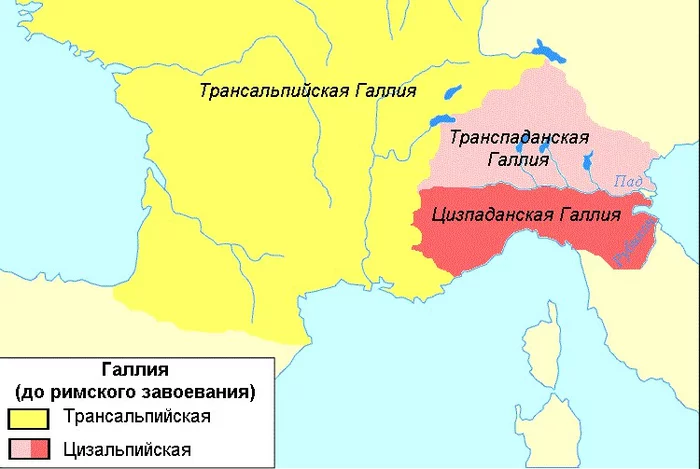
\includegraphics[scale=0.5]{kimres/1574758657154051178.png}
	\label{fig:kimr4} % Unique label used for referencing the figure in-text
	%\addcontentsline{toc}{figure}{Figure \ref{fig:placeholder}} % Uncomment to add the figure to the table of contents
	\caption{Транспаданская Галлия. }
\end{figure}

Марий соединил свои войска с войсками Катула и в очередной раз переизбрался на консульство. Катула же оставил при себе. С одной стороны, победы Мария на фоне поражения коллеги смотрелись ещё круче, с другой — если его убрать, то аристократия начнет бурлить и может подкинуть очередного знатного дебила, который в самый неподходящий момент начнет тупить и не выполнять приказы, как оно уже не раз бывало. Катул же о своих талантах был вообщет и сам невысокого мнения, а после прошлогодней кампании окончательно сдулся и был готов делать что скажет Марий без особой внутренней ломки. Поэтому весной 101г до н.э, когда кимвры опять сдвинулись с места, им противостояла уже монолитная армия с единым командованием, плюс у них в активе было одно вырезанное без особых проблем германское племя, а значит и вера в то, что количество фрагов можно будет удвоить в ближайшее время.


За счет того, что варвары, после легкой победы над Катулом, частично разбрелись по долине По, а Марий наоборот, за зиму усилил армию и добрал союзные контингенты, у римлян на этот раз был паритет в силах или даже численное преимущество, поэтому они сами пошли в наступление. Войдя в Транспаданскую Галлию, легионы начали маневрировать против германцев, отрезая тех от снабжения, и, одновременно, Марий вступил в переговоры с их вождем, вызывая того на "стрелку" на поле рядом с городом Верцеллы. Зачем? Дело в том, что Марий уже тогда понимал, что скоро от него попытаются избавится, уж больно он всех задолбал, и чтобы выжить на политическом поле, ему нужна славная, безоговорочная победа. Он мог бы, как и в прошлый раз, заставить варваров истощить силы, постепенно вымотать и перерезать, но это не ярко и не интересно. В общем, Марий договаривается с варварским вождем о бое недалеко от Верцелл, и в нужный момент приведя туда всю свою армию. Катула с его легионами он поставил в центре, как наиболее слабую часть армии, а на флангах расположил свои собственные, уже ветеранские легионы и кавалерию. Варвары, с классической для себя незатейливостью, выстроились чем-то средним между толпой и фалангой. А далее точь-в-точь повторился сценарий, который Ганнибал за сотню лет до описываемых событий провернул с самими римлянами при Каннах — варвары вломились в центр римского строя, Марий дал им время там завязнуть, а потом двинул вперед свои легионы, стоящие на флангах, тем временем отогнав конницей вражеских всадников. Легионы Мария смяли фланги германцев и зашли им в тыл, попутно взяв штурмом лагерь, а затем началась резня, где варварская армия, в полном окружении и сжатая на очень узком пятачке земли была просто расстреляна и уничтожена. На этом нашествие кимвров закончилось, как и сама Кимврская война. Третья группа варваров, которая так и не успела к тому времени перейти Альпы, просто рассеялась, когда до них дошли сведения о судьбе первых двух.


На этом столь подробную хронику событий можно прекратить, и промотать вперед целых десять лет римской истории, до следующей войны. И посмотреть как их провели все основные участники истории:

\begin{figure}[h!tb]
	\centering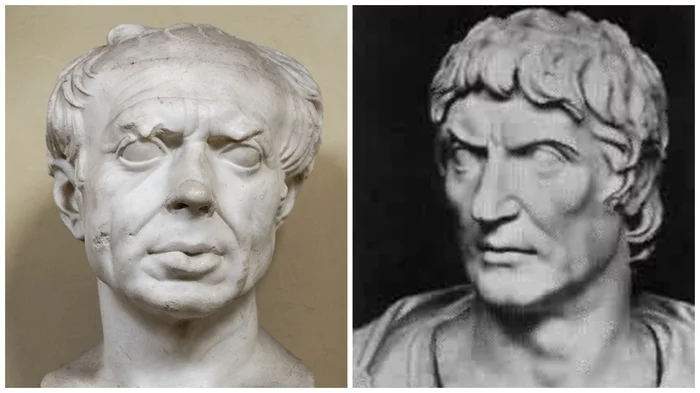
\includegraphics[scale=0.6]{kimres/157475883618344045.png}
	\label{fig:kimr5} % Unique label used for referencing the figure in-text
	%\addcontentsline{toc}{figure}{Figure \ref{fig:placeholder}} % Uncomment to add the figure to the table of contents
	\caption{Слева Гай Марий, справа Луций Корнелий Сулла. }
\end{figure}
Что касается Мария, то столь славные победы ему не помогли, в конечном итоге, и его партию вскоре разогнали, а сам он отправился в добровольное изгнание, в основном для того чтобы не попасть под суд и не отправиться в "недобровольное". Лишив Мария реальных рычагов управления Республикой, оптиматы всё-таки забоялись трогать его самого, так как слишком уж силен был тот героический ореол, который к нему прилип после разгрома германцев. Плюс, его ветераны уже тогда начинали занимать место в римской политике и становиться опорой партии популяров. До прямого участие легионов в политической жизни ещё очень далеко, но откровенных нападок на своего командира они могли не простить уже сейчас, а кому охота устраивать гражданскую войну на ровном месте? Поэтому Марий просто уезжает путешествовать по миру.


Сулла же, показав себя первоклассным военным, постепенно входит в круг высшей римской аристократии. Им нужен был свой, лояльный противовес Марию, на случай всяких неожиданностей. Чтобы, если вдруг набегут опять какие-то германцы, не пришлось бежать к старику, вручать ему армии, и на коленях просить "Мариюшка, защити нас, убогих, не можем без тебя, все битвы просираем и воевать совсем не умеем!". В отличии от Мария, слава которого за это десятилетие сильно поблекла, Сулла наоборот, очень сильно, хоть и без резких скачков, поднялся, и их, в принципе, можно было рассматривать в одной весовой категории. Успел понаместничать в Киликии, побыть претором Рима, принять персидских послов и повоевать с Тиграном II (союзником Митридата). В общем, отлично проводил время.


Но тут, ВНЕЗАПНО, ситуация как-то одномоментно рухнула в пропасть, а Республика опять оказалась на краю гибели. Началась Союзническая война. Когда я описывал сбор Марием армии, то просил запомнить его обещания гражданства союзникам за помощь. Община отдавала под рекрутинг 10\% своего мужского и пригодного к армейской службе населения, за это получала гражданство. Союзники, в целом, свои обязательства выполнили, мобилизовались, прошли тяжелую римскую армейскую школу, победили германцев и были распущены по домам. Сенат тогда дрожал от ужаса и не глядя подмахивал всё что Марий ему преподносил. А потом оптиматы очнулись, подумали, и просто утопили указы Мария в своей бюрократии на долгие десять лет.


Чтоб читатель понимал всю интересность ситуации, надо отметить устройство самой Италии непосредственно перед войной. В свое время Рим одну за другой подчинял себе народности полуострова и заключал с ними договора. Суть такова: они предоставляют союзные контингенты в армию (те самые войска поддержки), платят налоги, идут в русле римской политики, ну и всё, в принципе. Ещё им отрезали какую-то часть земель в пользу Рима, а остальное оставляли в собственности общин. Полисная система им в этом помогала, в том плане, что Рим мог заключать договора с каждым конкретным городом на индивидуальных началах, не давая тем же самнитам или этрускам возможности создать свою федерацию городов, достаточно крупную, чтобы противостоять Риму. Окрестности Рима гражданство уже давно получили (например, Квинт Серторий происходил из земель сабинян, которые Римом были завоеваны в 290г до н.э., а гражданство получили в 268г до н.э, после чего тихо-мирно утратили самобытность и растворились в римском этносе. К 1в до н.э. отличить жителей Сабина от жителей Рима не смог бы даже мамкин антрополог со штангенциркулем наперевес), а вот области Северной и Южной Италии состояли из союзных земель почти полностью, и на них же падали основные несправедливости и поборы. Рим активно строил там колонии из граждан Рима, являющихся этакими аванпостами на их территориях, но вот включать давно уже романизировавшихся италиков в свой состав не спешил. Тут же надо отметить и подушный налог на общины, а также общую проблему всей Италии — экономический кризис.


После Второй Пунической войны в Риме образовались несколько десятков олигархических семей, пришедших к власти (те самые оптиматы), которые начали проворачивать нехитрую схему получения гешефта — спонсируем завоевательные войны и получаем как прямой профит, так и рабов, причем сотнями тысяч чуть ли не ежегодно, с каждой большой войны. Затем проворачиваем в Сенате хитрую схему, и общинные земли (то есть те земли в Италии, которые Рим отжал у италиков в свое время, и они как бы общие) берем в аренду, попользоваться. На них строим здоровенные колхозы, загоняем туда тысячи рабов, и они пашут, производят всякое, а мы гребем гешефт. Земля бесплатная, рабы почти бесплатные, в итоге рентабельность производства абсолютно дикая, а доходы огромные. На полученные деньги отжимаем ещё земель, уже у самих союзников или просто разоряющихся римских граждан, строим там ещё колхозов, и так по кругу. Это обогатило олигархов, но загнало хозяйственную жизнь Италии в полную жопу, там стало нерентабельно производить вообще ничего. И если мелкие собственники земли из римских граждан ещё как-то держались на плаву, в силу льгот от государства, то на общины италиков всем было насрать, и они стремительно нищали. На фоне богатеющего с каждым годом Рима выглядело это совсем не по союзнически. Ну и поражение в правах, конечно. Со свойственным Риму снобизмом, жители Италии делились на граждан, не совсем граждан и вообще не граждан, и по этому признаку дискриминировались как отдельные личности, так и целые народы. Вот такой набор факторов.


Особый баттхерт испытывали жители Южной Италии. В период Второй Пунической войны именно тут Ганнибал смог опереться, перетащить на свою сторону несколько крупных городов, и долгие почти два десятилетия его оттуда не могли сковырнуть. Когда "Великий Пуниец" всё таки вернулся в Африку, а римляне смогли зачистить Италию, на поддержавшие его области обрушились секторальные санкции, как в моменте (массовые расстрелы и депортации в стиле усатого семинариста), так и в долгосрочной перспективе (более жесткие условия оккупации). И хоть прошло уже больше ста лет, но "осадочек остался". Плюс, тут сильнее чувствовалось греческое влияние. До прихода римлян именно греки заспамили всё побережье Южной Италии своими колониями. Ну и регион был просто богаче, более густо заселен, сильнее ориентирован на на торговлю и производство, по которым кризис бил в первую очередь. Если на севере грязные и необразованные этрусские пастухи пасли овец себе, и не сильно парились по сложным материям типа гражданских прав, то Южная Италия откровенно бурлила.


\begin{figure}[h!tb]
	\centering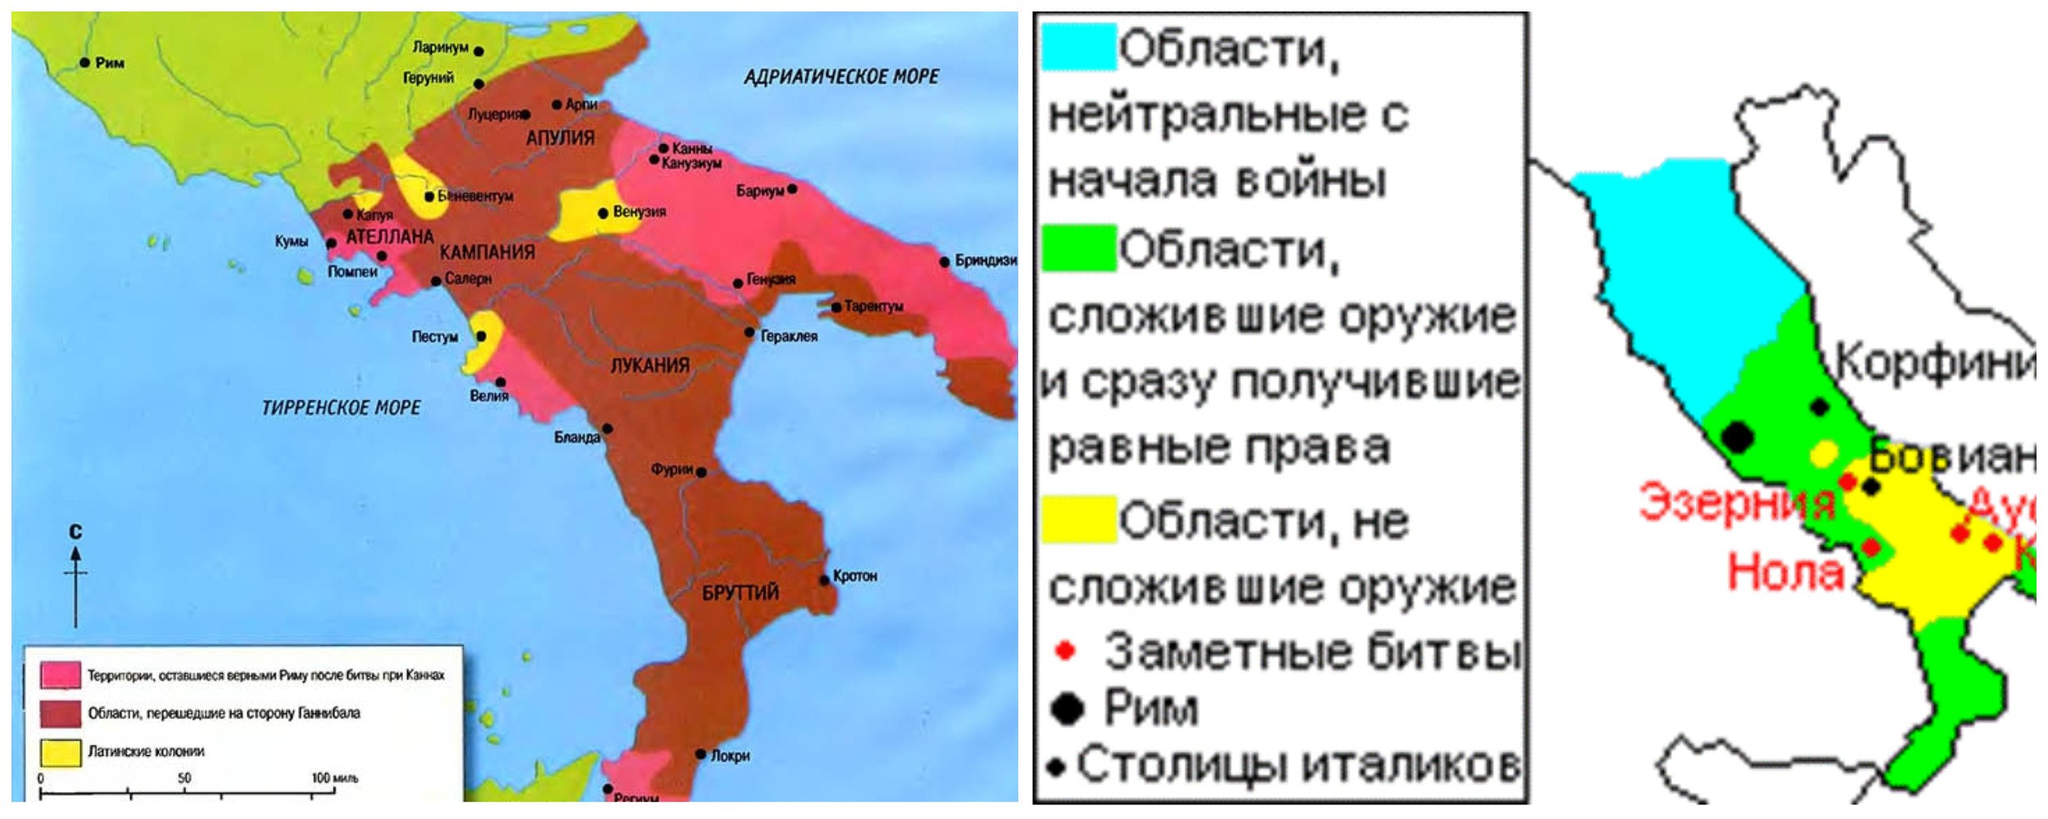
\includegraphics[scale=0.2]{kimres/1574759302180267294.png}
	\label{fig:kimr6} % Unique label used for referencing the figure in-text
	%\addcontentsline{toc}{figure}{Figure \ref{fig:placeholder}} % Uncomment to add the figure to the table of contents
	\caption{Слева карта перешедших на сторону Ганнибала територий (коричневая), справа восставшие общины в Союзнической войне (зеленая и желтая область). Совпадение? Не думаю.}
\end{figure}
А теперь вишенка на торте. В этих самых условиях Рим, который весь из себя непобедимый, умудряется просрать кучу сражений германским племенам, несколько раз находясь на краю гибели, а потом бежит к италикам в полном ужасе, умоляя помочь, "ведь Италия это наш общий дом, а мы все братушки-братушечки", щедро раздает обещание прекратить дискриминацию, уравняв всех в правах. Набирает из италиков новую армию (у Мария союзных контингентов было примерно половина, и это только официальные союзники. Немало италиков просто служило в легионах в частном порядке, за обещанное гражданство для себя лично), их кровью заливает германское вторжение, а затем... А затем из под шконки выползает оптиматская партия, которая там сидела в 105-101г до н.э, сливает Мария (который, отметим, был намерен честно выполнить те обязательства, которые принял на себя. Не просто так, канешн, это бы дало ему огромное количество благодарных клиентов и упрочило власть настолько, что с ним уже ничего невозможно было бы сделать легальными средствами), топит все обещания в канцелярщине, и, мол "идите обратно в стойла, друзья и союзники римского народа, чето вы какие-то излишне охуевшие, много просите".


А люди, которые воевали вместе с Марием — никуда не делись. Они вернулись домой, получив боевой опыт и приобретя самосознание в стиле "мы спасли Италию, без нас Риму пришел бы конец". Вот, таковы предпосылки этой войны, извиняюсь за долгое вступление. Все таки, самым важным тут была эта "революция сознания", когда римляне сами дали италикам почувствовать себя не просто равными себе, но ещё какбы остались им морально должны. И в стойла после этого им совершенно не хотелось...


Про саму войну поговорим как-нибудь потом. Этот текст -- составная часть моего Римского цикла, нужная чтобы на пальцах пояснить причины, ход и следствия Кимврской войны. Как видите, она уже вылилась в Марианскую реформу и войну Союзническую, и это только первый уровень последствий. Затем она, буквально ещё через пару лет, выльется в гражданскую войну межу Марием и Суллой. В немалой степени отсюда растут уши у Серторианской войны, да и Митридатовы войны тоже совсем близко. А там уже и до Цезаря недалеко. Вот так бывает, набегут к тебе варвары, ты позовешь компетентного специалиста чтобы их прогнать, а он тебе дом подожжет на, считай, семьдесят лет, лол. 
